\chapter{Cryptography}
	\label{ch:Cryptography}
	\section{Introduction to Cryptography}
		%Resource: http://www.thegeekstuff.com/2012/07/cryptography-basics/
		%Resource: http://www.pgpi.org/doc/pgpintro/
		%Resource: http://cacr.uwaterloo.ca/hac/
		Cryptography is the only means of securely transmitting data across a network. 
		It is also the only means of ensuring that data cannot be read by any individual who has access to a storage medium. 
		Thus, it is one of the more important concepts in computational security. 
		Without cryptography, nothing can be confirmed and nothing is secure. 
		However, even with it, it is easy to get wrong. 
		This section will discuss the basic ideas of cryptography without the mathematical background or the algorithmic understanding. 
		It will provide an overview on the requirements for a secure transmission. 
		The technical details of this will be presented in the later sections of this chapter. 
		These details for the specific standards that are used later in this chapter can be found in the FIPS released by NIST.\footnote{\url{http://csrc.nist.gov/groups/STM/cmvp/index.html}}
		\subsection{Key Terms}
			There are a number of terms within Cryptography that you will need to understand before you will understand the field.
			These terms are used to explain the goal or use of a particular part of cryptography\footnote{\url{http://www.thegeekstuff.com/2012/07/cryptography-basics/}}
			\begin{description}
				\item[Plaintext]
					The original message that is to be sent, signed or checked. 
					This is the message that the user or protocol writes to be transmitted to the other host or stored. 
				\item[Ciphertext]
					This is the cryptographically ``secure'' form of the plaintext above. 
					This means that the plaintext has gone through a cryptographical algorithm and is now enciphered within this text. 
				\item[Encryption]
					Conversion from a readable plaintext into an unreadable ciphertext. 
					This is mainly used to gain privacy in either storage or transmission. 
					This process will also come with a key or key pair that is used to encrypt the plaintext. 
				\item[Decryption]
					The process of converting an unreadable ciphertext into a readable plaintext. 
					This is used to allow the decrypting party to read the text. 
					This process will also need either the key, or the second half of the key pair. 
				\item[Authentication]
					This is the act of ensuring that the message received came from the sender claimed by the message. 
					This is based on an action that the receiving party knows only the sending party should be able to do. 
					Usually, this is done through signing with a private key. 
					The signature is then checked with the public key. 
				\item[Integrity] 
					This is the process of checking that the message received has not been altered in transmission. 
					This check is done on receipt of the message, ensuring that any changes in transmission are noticed. 
					Hashing algorithms such as SHA and MD5 are usually used for this process. 
				\item[Non-repudiation]
					Messages that are sent can be traced back to the original source. 
					That source cannot say that they did not send the message as a digital signature has stated their action. 
					This is done in much the same manner as authentication. 
				\item[Hash]
					This is a ``one way'' algorithm that takes a message an converts in into another form. 
					The basis of this is that there should be no way to reverse the algorithm given the output hash. 
					Furthermore, there should be minimal collisions with other messages. 
				\item[Keyspace] The maximum number of possible keys that a cryptographical algorithm could use. 
			\end{description}
		\subsection{Types of Cryptography}
			This section will discuss the three main types of cryptography: secret key, public key and hashing. 
			\subsubsection{Secret Key Cryptograhpy}
				This form uses a single key that all accessing parties must have. 
				The keys complexity---along with the strength of the algorithm---determines the strength of the encryption.
				Due to the use of the same key at either side of the process, this is also commonly known as ``symmetric key encryption. 
				While this type of encryption is usually faster, is poses the problem of getting the key to the other user. 
				This problem is largely alleviated through the use of public key cryptography and key exchange algorithms.
				An example of this process can be found in Figure \ref{fig:SymmetricKey}
				\begin{figure}[htb]
					\centering
					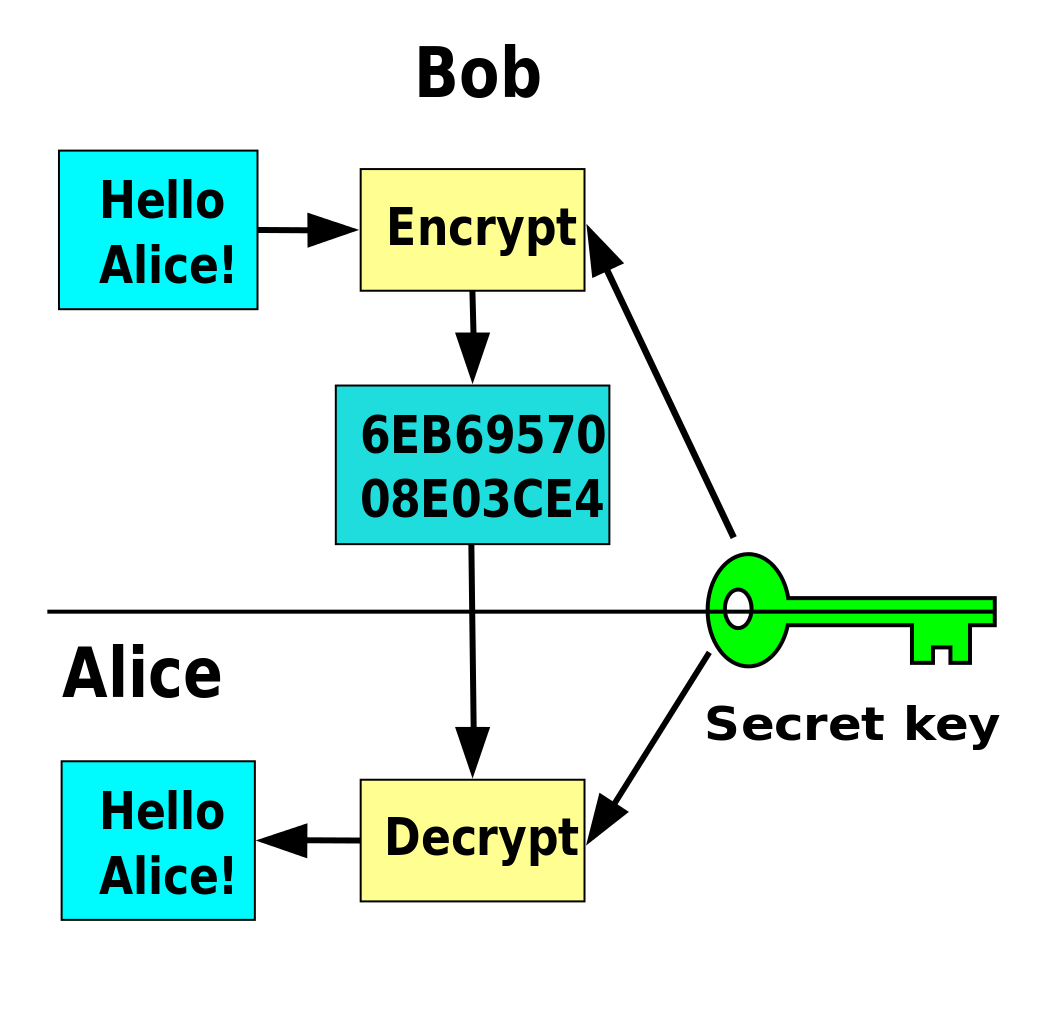
\includegraphics[scale=0.25]{./SymmetricKey.png}
					\caption{Symmetric Key Cryptography Process}
					\label{fig:SymmetricKey}
				\end{figure}
			\subsubsection{Public Key Cryptography}
				Unlike symmetric key cryptography, public key cryptography uses two keys, one stored at each party. 
				These two keys are completely different. 
				They are designed in such a way that given one of them, you should not be able to determine the other. 
				These two keys each have a name and a set of properties. 
				The key used to encrypt the data is known as the public key. 
				It can be read by anyone, as it will not give them access to the data. 
				The key used to decrypt the data is known as the private key. 
				This key will be securely stored on the receiving computer and should never be transmitted. 
				While this solves the problem of key exchange, it is significantly slower. 
				An example of this process can be found in figure \ref{fig:PublicKey}
				\begin{figure}[htb]
					\centering
					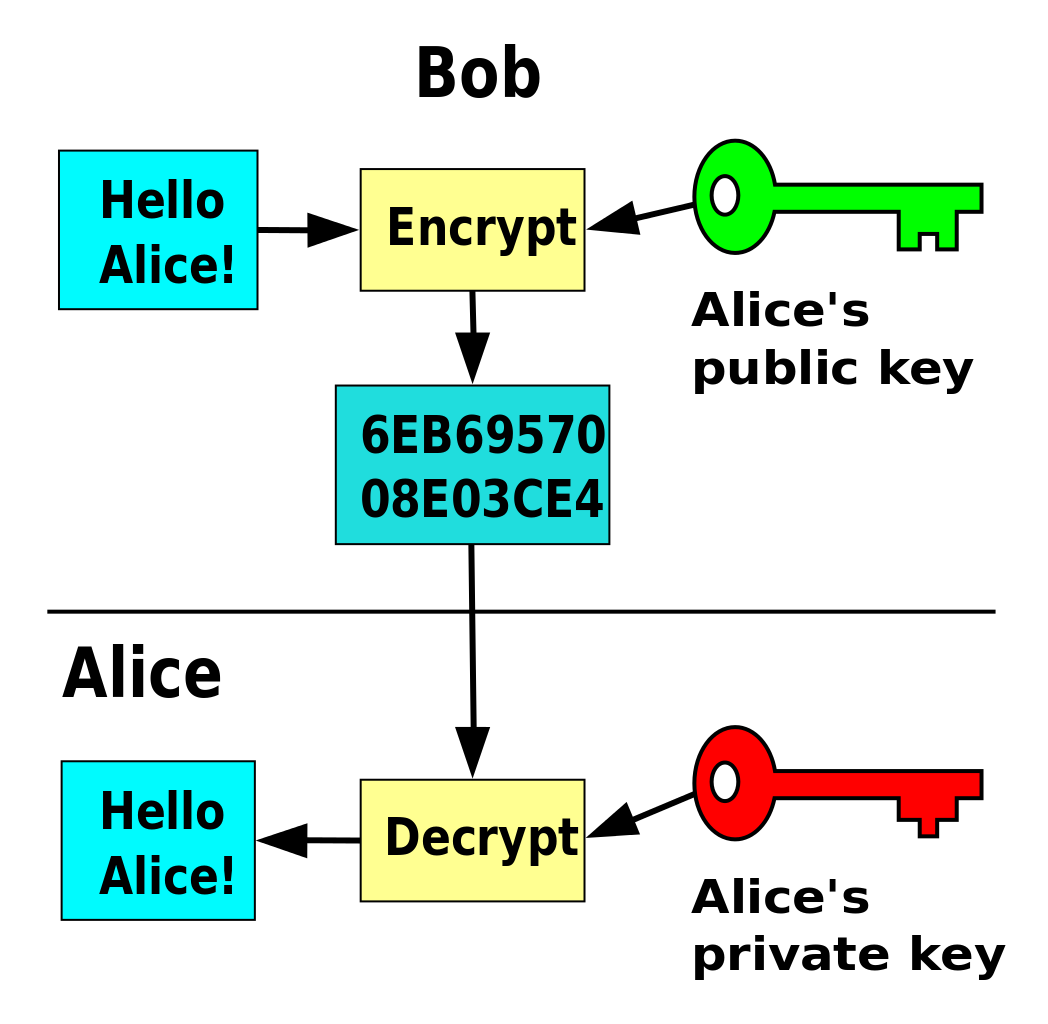
\includegraphics[scale=0.25]{./PublicKey.png}
					\caption{Public Key Cryptography Process}
					\label{fig:PublicKey}
				\end{figure}
			\subsubsection{Hashing}
				Hashing does not involve a key, though it may use a salt to ensure the uniqueness of the hash. 
				This process creates a fixed length hash value which represents the plain text message. 
				However, there is no way of taking this hash value and algorithmically decoding the plain text from it. 

				This process is often used in checking that the correct data was transmitted unaltered. 
				It can further be used for the storage of items that need to be checked but should not be stored in plain text. 
				An example of this would be the storage of passwords. 
				
				An example of the hashing process can be found in figure \ref{fig:HashingProcess}
				\begin{figure}[htb]
					\centering
					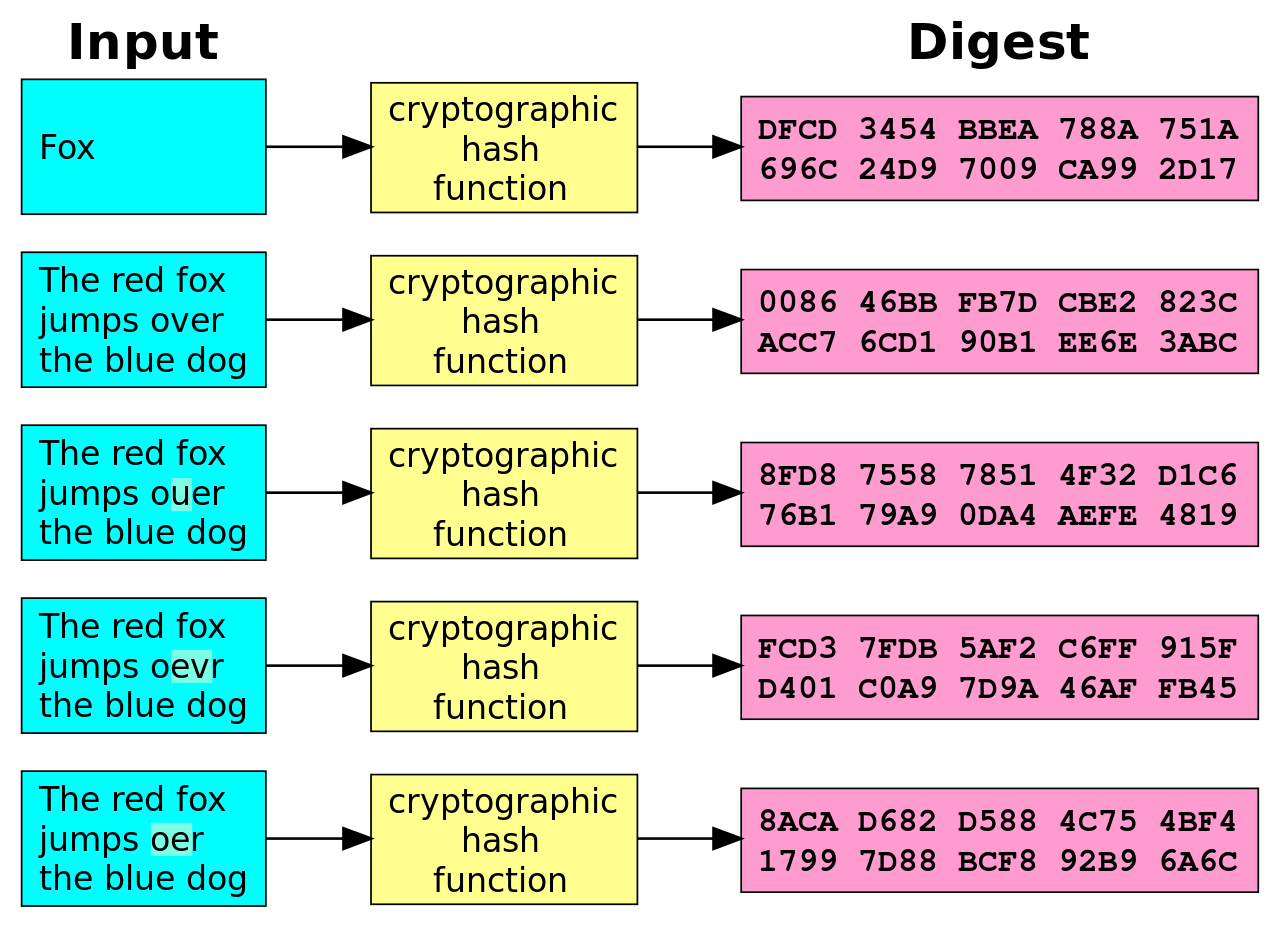
\includegraphics[scale=0.25]{./HashProcess.png}
					\caption{Hashing Process}
					\label{fig:HashingProcess}
				\end{figure}



		\subsection{Basic Cryptography}
			Cryptography has been around since ancient times. 
			However, it has only been with the introduction of the modern computer that it has become complex and of a high standard. 
			This is because computers are good at breaking weak cryptography, that was the whole purpose of the first digital computer created by Alan Turing and his team at Bletchley Park. 
			This first machine was designed to break the German Enigma Code and was exceptionally successful at it. 

			Basic encryption should not be used in the modern world. 
			It is not the type of encryption that would survive seconds against a well programmed computer. 
			Rather, it is the type of encryption that worked well for the Romans on the battlefield, well before the other commanders had heard of such techniques. 

			\subsubsection{Caesar's Cipher}
				This is the first algorithm that we will discuss. 
				It has little current use, as it's keyspace is 25, however, it serves as a good learning tool. 

				Caesar's Cipher is a simple substitution cipher\footnote{\url{http://www.pgpi.org/doc/pgpintro/}}. 
				This means that the key is simply a number that the alphabet used is shifted by. 
				Then, each letter in the plain text is substituted for the equivalent letter in the shifted alphabet. 
				This process can be seen in figure \ref{fig:CaesarsCipher}
				\begin{figure}[htb]
					\centering
					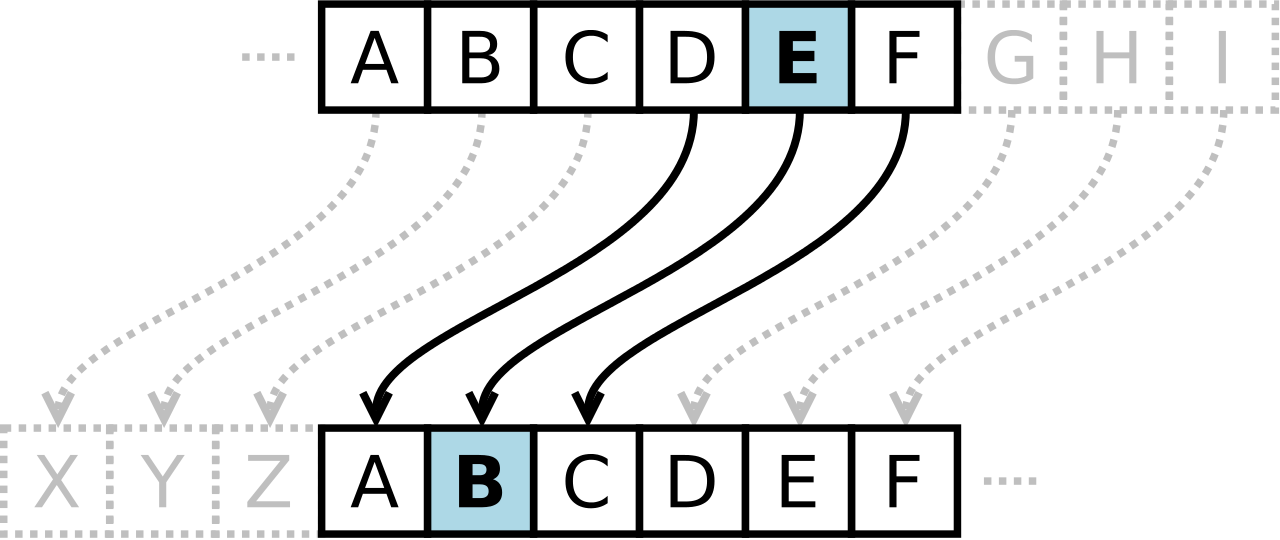
\includegraphics[scale=0.25]{./CaesarsCipher.png}
					\caption{The Method used for a substitution cipher}
					\label{fig:CaesarsCipher}
				\end{figure}
			\subsection{XOR Cryptography}
				In the same light as the Caesar's cipher, XOR should not be used when you are looking for security. 
				However, it is a stronger algorithm than the substitution cipher shown above. 
				This is due to the fact that the key which can be used for XOR can be as long as the plain text. 

				While stronger than a substitution cipher, XOR still has a number of issues. 
				Foremost is the fact that it is easily reversible. 
				This means that given a known part of the plain text, the key can be deduced. 
				This becomes most obvious when the plain text has a section of null bytes. 
				These bytes will output as the key when passed through the algorithm. 
				Thus, if the attacker may know any part of the plain text, or can control it, XOR is just as weak as a substitution cipher. 

				Furthermore, there is no key chaining done in this algorithm. 
				Thus, if a short key is used, common parts of the plain text will be output in a similar way. 
				This means that images could still show detail and the cipher text is vulnerable to statistical analysis. 

				The XOR algorithm works by running a binary exclusive OR (see chapter \ref{ch:GeneralKnowledge}) 
				over each bit within the plain text and key. 
				The key is looped around, such that each time it gets to the end it links back to the start. 

			\begin{figure}[htb]
				\centering
				\begin{tabular}{| l | l | l |}
					\hline
					\textbf{Plaintext} & \textbf{Key} & \textbf{Ciphertext} \\ \hline
					10101011101010 & 10101110 & 00000100111101 \\ \hline
					00000000000000 & 10101110 & 10101110101011 \\ \hline
					10101011101010 & 00000000 & 10101011101010 \\ \hline
				\end{tabular}
				\caption{XOR Cryptography Example}
				\label{fig:XORExample}
			\end{figure}
			\subsubsection{Encodings}
				Many people confuse encoding for encryption. 
				This confusion can lead to information being leaked, as encoding will not provide any protection. 
				To the untrained eye, these two look similar. 
				However, there are differences that should be understood and can be used to detect which is being used. 

				Encoding, much like encryption and hashing uses a known algorithm. 
				However, unlike encryption, encoding does not use a key. 
				Furthermore, unlike hashing, encoding is not one way. 
				This means that encoding can quickly and easily be returned to plain text as the means of returning is embedded within the algorithm.

				Encoding works by specifying a known character set and mappings amongst this. 
				For example, the binary data that forms this document in encoded as UTF-8, which you read as text. 
				However, this can be done in a different manner. 
				For example, this text could be encoded as a number, or as base 64. 

				Each of these different types of encoding has some part which can be used to determine what type of encoding is used. 
				For example, simple text will usually be encoded as ASCII. 
				Higher characters will have to be encoded as UTF-8 or UTF-16. 
				Numbers can be encoded as decimals, or in a higher base such as 16 or 64. 
				Table \ref{tab:Encodings} contains a list of the names and look of many common encodings. 
				\begin{table}[htb]
					\centering
				\begin{adjustbox}{max width=1\textwidth}
					\begin{tabular}{| l | l |}
						\hline
						\textbf{Name} & \textbf{Encoded Text Example} \\ \hline
						ASCII, UTF-8 etc & This is normal text \\ \hline
						Hexadecimal, base 16 & DEADBEEF, 46DEAC46BC \\ \hline
						Base 64 & YW55IGNhcm5hbCBwbGVhcw== \\ \hline
					\end{tabular}
				\end{adjustbox}
					\caption{Common Encoding Examples}
					\label{tab:Encodings}
				\end{table}
	\section{RSA}
		
		\subsection{\{N : e : c \} Format}
		\subsection{Common Flaws}
		\subsection{Key Recovery}
	\section{Merkle-Hallman Knapsack Cryptosystem}
	\section{Key Exchange}
		%Resource: http://security.stackexchange.com/questions/45963/diffie-hellman-key-exchange-in-plain-english
	\section{Server Authentication}
	\section{Rotational Algorithms}
	\section{Utilizing Cryptography in Python}
	\section{Poor Cryptography Implementations}
		\subsection{DES Weak Keys}
	\section{Eilliptic Curve Encryption}
		\subsection{Common Attacks}
	\section{Hash Cracking}
		Hashes are used in many situations to store passwords. 
		This is done because the hashing algorithm is a one way action, meaning that there is no easy way to calculate the password from the hash. 
		Due to this, the means of authentication on most programs is done by hashing the entered password and comparing it to a stored hash. 
		If the two match, it is likely---though not guaranteed due to collisions---that the password is the same. 
		While this may sound like it makes attacking these targets hard, it is far from being unsolvable. 
		Tools such as ``John the Riper'' and ``Hashcat'' can be used to compute hundreds of thousands of hashes per second, which can then be compared with the given hash. 
		This makes hash cracking a matter of time and dictionary crafting. 
		\subsection{John the Riper}
			While there are many tutorials\footnote{\url{http://openwall.info/wiki/john/tutorials}} on the usage of John the Riper (John) which go into specific detail, this section will explain the basic usage of the tool. 
			Before starting, check that the version of John which you have installed is correctly compiled for your system, you may want to enable options such as GPU cracking, which needs to be done at compile time. 
			What follows is a list of common commands for use with John:
			\begin{description}
				\item[-single]
					The simplest means of attacking a hash. 
					This mode uses only a basic word-list and very few rules. 
					Thus it is not recommended for anything but the most basic attacks. 
				\item[-wordfile:]
					Uses the word-list specified directly after the colon. 
				\item[-rules:]
					Specifies the mutation rules for the given word-list. 
					These can be used to create a dictionary with substitutions, such as 1337 speak. 
				\item[-incremental:]
					This, along with options such as ``alpha'', ``digits'' or ``lanman'' will give you a brute force of letters, numbers or both with some special characters respectively. 
				\item[-external:]
					Allows the use of pre-configured modes, which can be powerful if used or modified correctly. 
					%TODO: add more to this and rules. 
				\item[-restore:]
					Will start a crack part way through based on a restore file created by a previous session. 
				\item[-sesion:]
					Used to name the restore file that will be created when the session is broken. 
				\item[-status:]
					Shows how far into the crack a previous session was stopped. 
				\item[-show]
					Shows how many passwords within a file have been cracked and how many remain. 
				\item[-format:]
					Specify the hash format (such as SHA512) which the hash to crack was created with. 
			\end{description}
			
		\subsection{Hashcat}
			Hashcat was started due to the fact that at the time, tools such as John the Riper did not make proper use of multi-threading. 
			This has been expanded to include GPGPU processing using tools such as openCL and CUDA, and has made hashcat one of the fastest hash cracking tools currently available. 
			Both Hashcat and the newer oclHashcat use the same input files and command syntax. 
			However, oclHashcat will conduct the crack on the GPU installed on the system, rather than the slower CPU. 

			Hashcat uses a number of modes to allow it to crack hashes. 
			Each of these modes has a number of specific properties which make it better at a given type of attack. 

			\subsubsection{Mask Attack}
				This attack, while similar to a brute force attack, uses a mask to reduce the possible character set of the attacks.\footnote{\url{http://hashcat.net/wiki/doku.php?id=mask_attack}} 
				Rather than run through every possible permutation of the character space for every character in the password, the mask attack requires that the user input some details of the characters within the password. 
				
				When using this mode, for each position within the password, we need to create a mask using either the character sets outlined in table \ref{tab:HashcatMaskCharSets} or a custom character set defined before starting. 
				\begin{table}[htb]
					\centering
				\begin{adjustbox}{max width=1\textwidth}
					\begin{tabular}{| l | l |}
						\hline
						?l & abcdefghijklmnopqrstuvwxyz \\ \hline
						?u & ABCDEFGHIJKLMNOPQRSTUVWXYZ \\ \hline
						?d & 0123456789 \\ \hline
						?s & <space>!"\#\$\%\&\verb!'()*+,-./:;<=>?@[\]\^_`{|}~}! \\ \hline
						%?s & Special Characters \\ \hline%TODO: Have this print the characters. 
						?a & \verb+?l?u?d?s+ \\ \hline
						?b & 0x00 - 0xff \\ \hline
					\end{tabular}
				\end{adjustbox}
					\caption{Hashcat Mask Mode Built in Character Sets}
					\label{tab:HashcatMaskCharSets}
				\end{table}
				Attacks in this mode are limited by the length of the mask given. 
				This means that if you give a mask with 8 character spaces, but have a password which is 6 characters long, you will be unable to crack it. 
				Due to this, the ``\verb+--+increment'' flag was created. 
				Furthermore, a list of standard character sets for multiple languages can be found in ``/usr/share/hashcat/charsets/''.

				Another means of creating this attack mode is to use a Hashcat Mask File. 
				These files contain a number of masks and the custom character sets which are used within them, in order to run attacks which are regularly repeated. 
				To use one of these files, run Hash cat with the arguments ``-a 3 <hash file> <mask file>''.

			\subsubsection{Dictionary Attack}
				In this attack, a dictionary or word list is created to be utilized within the attack. 
				This dictionary can either be one that you found on the system or one that was created specifically for the job. 
				Due to the limitations of this attack, it is recommended that it is either used with a specifically generated dictionary, which can be done by a program such as John the Riper or
				a can be manually written through the use of a python script. 
				This type of attack may be the first that you use, as it will likely be the quickest attack. 
			\subsubsection{Combinator Attack}
				In this attack, each word of a dictionary is appended to each word in a second dictionary. 
				This will catch many passwords which use two simple words, as long as the dictionary is well written. 
				However, if the dictionaries that you are using have already been enumerated in such a way, it will likely not produce useful results. 
				Furthermore, this attack will not run the words from each dictionary separately. 
				To use this attack, run the top command for GPU or the bottom command for CPU. 
				\begin{lstlisting}[style=CLI]
					$ oclHashcat64 -m 0 -a 1 <hash file> <dict1> <dict2>
					
					$ hashcat-cli64 -m 0 -a 1 <hash file> <dict 1 and 2>
				\end{lstlisting}
			\subsubsection{Hybrid Attack}
				This attack uses the concepts of both the combinator and mask attacks. 
				This means that you can specify a dictionary and have hashcat add the mask that you give to either the start or end of the word. 
				Using this means, you can easily run through passwords such as name and birth year combinations. 
				To conduct this attack, use the command:
				\begin{lstlisting}[style=CLI]
					$ oclhashcat -a 7 <mask> <dict>
					$ oclhashcat -a 7 <dict> <mask>
				\end{lstlisting}
				
		\subsection{Rainbow Tables}
			In both of the previous sections, we have been calculating the hashes which we are testing against the password hash on the go. 
			This means that we have to calculate the algorithm, sometimes multiple thousands of times, for each password we want to try. 
			There is another option: rainbow tables. 
			This method of cracking passwords allows us to have a precomputed list of hashes and their respective passwords, which we then simply search through. 
			This results in two significant differences:
			\begin{itemize}
				\item Password cracking takes seconds
				\item Your hard drive is full. 
			\end{itemize}
			However, these tables are not the be all and end all of hash cracking. 
			They rely on the hashes being computed either with no salt or with the same salt as the table, meaning that hashes generated using a randomized salt will not be vulnerable. 
			Furthermore, they rely on the attacker being able to find a table which will suit the password. 
			Thus, if your password is a 50 character essay with special characters, it will likely not show up in the table due to size constraints. 
			Such a table would have to contain $\approx2.49\times10^{66}$ password--hash pairs, resulting in a file size of $\approx2.6\times10^{44}$Yottabytes.
			Though this cannot be thought of as a limitation when compared to the two other methods, as for the same password, they would take $\approx5.2\times10^{52}$ years on 3 ATI HD7970 GPUs.\footnote{\url{https://litecoin.info/Mining\_Hardware\_Comparison}}
			At this point, even assuming Moore's law continues and Processing power becomes far cheaper, the password will not be cracked within a reasonable time frame. 

			It is for these reasons that rainbow tables are uncommonly used outside of cracking hashes from poorly implemented software with short passwords. 
			However, if you know that the character space is small, and either the passwords are unsalted or the salt is commonly known, rainbow tables are the best method if you have the storage space. 
		\subsection{Online Methods}
			With the rise of cloud computing and cheap server rental, many people have begun using tools such as Amazon Web Services to run crack servers. 
			This is done by deploying the tools shown above into a server which has been rented with multiple GPUs. 
			This server can then be optimized such that the cracking will properly utilize the GPUs of the machine as well as only calculating hashes that have a possibility of being correct. 
			Thus, as above, if you know that the hash will be within a given dictionary, or that it does not contain special characters, use these functions. 

			While this will work, and usually faster than using one's own computer, it is not as fast as a dedicated cracking cluster. 
			These clusters work by having a number of machines, each with the necessary hardware and software installed working together on the one hash. 
			Programs such as Hashcat can be used to control up to 125 GPUs across the cluster in order to crack the hashes you provide. 
			This method, while expensive and difficult to set up, is currently the fastest means of cracking a hash. 
			However, if you set your cracking program up properly, it will still likely beat this setup when it is brute forcing hashes. 
		\subsection{Salting}
			Many of the methods above become significantly more difficult when salting is introduced. 
			Normally, a hash will be produced by simply running a hash function on the password ($hash(pass)$). 
			However, when salting is implemented, the hash may be generated by adding either a known string or a random string---or sometimes both---to the password before passing it to the hash function ($hash(pass + "salt"$ or $hash(pass + rand()$).
			In either of these cases, the salt must be stored, which has led to split salting, using a random stored value or the users name/ID as well as a hard coded element. 
			This makes knowing the salt hard, but not impossible, as we can reverse engineer the code in order to determine the salting algorithm used and a simple ``strings'' on the compiled code will give us a hard coded salt string. 
			Nonetheless, these methods deter attackers from attempting to crack the hashes by limiting their choices and removing their ability to use rainbow tables. 
		\subsection{SHA}
		\subsection{Hash Collisions}
			Hashes, by their nature must have collisions. 
			This is due to the fact that they take a large amount of information and turn it into a string of a standard size. 
			For example, an SHA256 hash has a length of 65 and a character space of 36. 
			This gives $1.84\times10^{66}$ possible values. 

			This is the basis for collisions. 
			Consider that there are vastly more than this number of items that can be hashed, 
			If this is true, some of these items must have the same hash value as other items.
			Furthermore, if you can find a collision with the item you are testing, you need only pass that collision, rather than the item itself. 

			This is the exact reason hashing algorithms such as MD5 are being replaced with SHA512. 
			It is now easy to find a collision value for the smaller key space MD5, meaning that using it for secure storage or any other purpose is near pointless. 

			Table \ref{tab:HashCollisions} contains the maximum number of hash values for common hash types.
			\begin{table}[htb]
				\centering
				\begin{adjustbox}{max width=1\textwidth}
				\begin{tabular}{| l | l |}
					\hline
					\textbf{Hash Type} & \textbf{Number of Values} \\ \hline
					SHA256 & $1.44\times10^{102}$ \\ \hline
					SHA512 & $5.79\times10^{201}$ \\ \hline
					SHA1   & $6.4\times10^{64}$ \\ \hline
					MD5	   & $2.28\times10^{52}$ \\ \hline
				\end{tabular}
			\end{adjustbox}
				\label{tab:HashCollisions}
				\caption{Number of Possible Hashes for Different Algorithms}
			\end{table} 
	\section{Challenges}
		\subsection{Hash Challenges}
			This first challenge is based on the \href{https://xkcd.com/936/}{xkcd comic ``Password Strength''.}
			The word-list for this challenge can be found by using the following command on kali linux:
			\begin{lstlisting}[style=CLI]
				$ head -n 20	/usr/share/wordlists/rockyou.txt
			\end{lstlisting}
			The password, hashed in MD5 and SHA256 can be found below. 
			\lstinputlisting[numbers=none,firstline=1,lastline=4]{./shellOut/hashChallenges.data}
			While you can complete this in any way you like, I recommend either using John's rules, or creating a custom word list and using Hashcat's hybird mode. 
			%Solution: "N1c0l3;7"

			The second challenge is based on an ATM keypad. 
			Through an image captured when the hash was pulled, it was determined that the only keys pressed were ``2, 4, 9 and 0''. 
			The password was also determined to be exactly 16 characters long. 
			Create a custom mask for Hashcat and solve this sha256 hash. 
			\lstinputlisting[numbers=none,firstline=6,lastline=6]{./shellOut/hashChallenges.data}
			%solution: "2490092442902942"

			The third challenge is based on using multiple dictionary words. 
			This is a common method used to create passwords. 
			I recommending using Hashcat in combinator mode to solve this SHA256 hash. 
			All the words necessary to solve this can be found in the rockyou word-list. 
			\lstinputlisting[numbers=none,firstline=8,lastline=8]{./shellOut/hashChallenges.data}
